\documentclass[10pt, a4paper]{article}

% Formatting
\usepackage{ctex}
\usepackage[margin=1in]{geometry}
\usepackage[titletoc,title]{appendix}

\usepackage[colorlinks,linkcolor=red]{hyperref}
\usepackage{amsmath,amsfonts,amssymb,mathtools}


\usepackage{graphicx,float}
\usepackage{xcolor}

\usepackage[ruled,vlined]{algorithm2e}
\usepackage{algorithmic}


\everymath{\displaystyle}


\usepackage{biblatex}
\addbibresource{references.bib}

% Title content
\title{数理统计学习笔记}
\author{慕弋云子}
\date{October 24, 2020}

\begin{document}

\maketitle

写这些东西主要是为了:
\begin{enumerate}
    \item 对于期末突击的同学们,可以迅速把握考点和做题技巧。
    \item 对于保研的同学、或者已经忘了概统内容甚至完全没学过的同学,这是一份很好的补充材料。
    \item 对于历年新生,可以做到不必听课,独立阅读文档并认真完成老师留的作业,就可以很好地完成数理统计的学习。
\end{enumerate}

阅读本文前你需要知道:
\begin{enumerate}
    \item 本人是2020级孙海燕老师班的学生,首先必须声明的是,孙老师讲得挺好的,对于许多概念有着深厚的理解和把握,授课思路也很清晰,但大抵是要照顾各种程度的学生,所以进度对于我这样的考研学生就显得有些“食之无味,弃之可惜”。于是,我便解锁了边听课边写作业的操作,争取每周形成此文,带领大家巩固每周的内容并更好地完成作业。
    \item 数理统计本身的知识内容就有很强的抽象性,配合北航这形式化的教材,自学起来实在困难。所以我们不如找一个生动形象、轻松诙谐的方式,来共同完成一些概念的学习。在这个过程中可能不那么严谨,但会更加直观。
    \item 本文内容都是基于孙老师课堂内容及所布置作业,每一大节对应每节课的作业。对于本文未提及的知识点和习题类型,学有余力者可自行学习;本文内容亦不对诸位读者的考试成绩负责,还望知悉。
\end{enumerate}\par
此外,本人对于latex的使用略有生疏,以及对于数理统计知识的掌握难免有疏漏之处,还望见谅。如对本文内容有任何问题,欢迎私信或发邮件至:gt3115a@163.com。

\section{充分统计量}
作业内容参考:1.11、1.12、1.14、1.15\par
第一次作业的内容全部都是关于充分统计量的。所以我们有必要来聊一聊什么是充分统计量。\par
但首先,我们还是来扯点儿别的,对数理统计形成一个初步的认识。\par 对于“不确定性”这个事情,一直以来就分为\textbf{频率派}和\textbf{贝叶斯派}两种观点。\par 比如频率派通过抛1000次硬币可以得出硬币是否均匀(或者均匀程度)这样的结论,从「自然」角度出发,试图直接为「事件」本身建模,认为硬币是否均匀这件事情是确定的,我们要做的只是大量实验去考察、近似参数,其代表性武器就是大数定律和最大似然估计。\par
而贝叶斯派则是以观察者的角度看问题,即先验知识可能是“这个硬币是均匀的”,然后做实验去验证这个结论,比如抛1000次只有20次朝上,最终得到的结论是「先验知识的可信程度」很低。贝叶斯学派并不试图说「事件本身是随机的」,或者「世界的本体带有某种随机性」,这套理论根本不言说关于「世界本体」的东西,而只是从「观察者知识不完备」这一出发点开始,构造一套在贝叶斯概率论的框架下可以对不确定知识做出推断的方法,其代表性武器就是最大后验估计、蒙特卡罗等。\par
而数理统计与这两派的关系相比大家也都猜到了:贝叶斯学派与频率学派是当今数理统计学的两大学派,基于各自的理论,在诸多领域中都起到了重要作用。贝叶斯派发展较新,因而人们也将频率学派称为古典学派,读者若有兴趣可以进一步探究一下贝叶斯这个神奇的人(他其实是个牧师)。\\\par
言归正传,「充分统计量」这个概念的产生,就是希望\textbf{在充分统计量确定之后,决定某个分布的参数就确定了。}具体来说,如果我们对某个分布进行一次采样,得到一系列样本,一般情况下每次采样得到的一系列样本都是互不相同的,比如某两次采样我们得到\{1,2,4,5\}和\{5,3,3,1\}。但我们发现,无论怎样采样,其内在的一些属性可能是不变的,最简单的比如说均值、方差等,当我们确定了这些量之后,就可以对参数做出推断,这就是充分统计量的想法。\par
这个时候你就会问了,这不是大海捞针吗,统计量那么多我怎么知道哪个是?实则不然,这其实是一件非常「套路」的事情。在介绍套路之前,还要介绍一个定理叫做\textbf{因子分解定理}。

\subsection*{Theorem 1 (因子分解定理)}
给一个不那么形式化的定义:一个关于参数$\theta$的联合分布$p(x;\theta)$,都可以被分解为两个部分的乘积。一个部分是与$\theta$无关的$h(x)$,是只含随机变量的函数;另一部分是无法被分解的,关于参数$\theta$和随机变量$x$的函数$g(T(x),\theta)$,其中$T(x)$是仅关于随机变量$x$的函数。\\\par

我们来举几个栗子,应该就更好理解了。\par
\textbf{栗子1.}假如我们求出联合概率分布是$p(x_1,x_2,...,x_n;\theta)=\theta^{n}\left(\prod_{i=1}^{n} x_{i}\right)^{\theta-1}$,那么定理所说的那两部分以及$T$分别是什么呢?\par 首先你会看到$\prod_{i=1}^{n} x_{i}$这个东西,然而它外边还套着一个$\theta-1$次方,所以这个东西实际上并不能被“分离”出来,所以说这一部分应该归属于$T$当中。最终我们应该得到,$h=1$,$T=\prod_{i=1}^{n} x_{i}$,$g=\theta^{n}T^{\theta-1}$。这里$h$、$T$、$g$都进行简写了,答题的时候最好写全一点:$h(x_1,x_2,...,x_n)$,$T(x_1,x_2,...,x_n)$,以及$g(T,\theta)$。
$h$经常就等于1,分不出来的时候可别愣着。\\ \par
\textbf{栗子2.}这回来一个双参数的。假如我们求出联合概率分布是:
\begin{center}
    $p\left(x_{1}, \cdots, x_{n} ; \mu, \sigma^{2}\right)=\left(\prod_{i=1}^{n} \frac{1}{\sqrt{2 \pi} \sigma x_{i}} \right) \exp \left\{-\frac{1}{2 \sigma^{2}} \sum_{i=1}^{n}\left(\ln x_{i}-\mu\right)^{2}\right\}$
\end{center}
那么$h$,$g$以及$T$又分别是什么呢?\par
别看$\sigma x_{i}$离得近,但它们是可以分开的;别看$\ln x_{i}-\mu$离得远,但他们应该被展开进而分离。所以我们应该对上述联合分布做变形,得到下面这个式子:\begin{center}$p\left(x_{1}, \cdots, x_{n} ; \mu, \sigma^{2}\right)=\left( \prod_{i=1}^{n} \frac{1}{\sqrt{2 \pi} x_{i}} \right) \sigma^{-n} \exp \left\{-\frac{1}{2 \sigma^{2}} \sum_{i=1}^{n} \ln ^{2} x_{i}+\frac{\mu}{\sigma^{2}} \sum_{i=1}^{n} \ln x_{i}-\frac{n \mu^{2}}{2 \sigma^{2}}\right\}$\end{center}\par
这样看起来就很清晰了。从左至右,一开始的$\prod_{i=1}^{n} \frac{1}{\sqrt{2 \pi} x_{i}}$与参数无关,应该被归为$h$中;$\sigma^{-n}$和最后的那个$-\frac{n \mu^{2}}{2 \sigma^{2}}$(事实上应该是$\exp \left\{-\frac{n \mu^{2}}{2 \sigma^{2}}\right\}$)则是属于$g$而又不属于$T$的那部分(这部分往往不一定好被分离出来);$\sum_{i=1}^{n} \ln ^{2} x_{i}$和$\sum_{i=1}^{n} \ln x_{i}$因为系数含参,显然它们都应该被归入$T$中。\par
这时候就有个问题,有两项都要被归入$T$中该怎么办?这时候就可以引入数对来表示,即$T(x_1,x_2,...,x_n)=(\sum_{i=1}^{n} \ln ^{2} x_{i},\sum_{i=1}^{n} \ln x_{i})$,并且我们用$T_1$表示前者,$T_2$表示后者。\par
最终,我们得到:
\begin{center}
$h=\prod_{i=1}^{n} \frac{1}{\sqrt{2 \pi} x_{i}}$,$T=(\sum_{i=1}^{n} \ln ^{2} x_{i},\sum_{i=1}^{n} \ln x_{i})$,$g=\sigma^{-n} \exp \left\{-\frac{1}{2 \sigma^{2}} T_1 +\frac{\mu}{\sigma^{2}} T_2 -\frac{n \mu^{2}}{2 \sigma^{2}}\right\}$。
\end{center} \par
\textbf{栗子3.}最后再举一个涉及区间的分布。现在我们考虑一个均匀分布$U\left(\theta_{1}, \theta_{2}\right)$,显然它的联合概率分布应该写成:
\begin{center}
    $p\left(x_1, x_2,...,x_n ; \theta_{1}, \theta_{2}\right)=\left\{\begin{array}{ll}
        (\frac{1}{\theta_{2}-\theta_{1}})^n & \theta_{1}<x_i<\theta_{2},\qquad i=1,...,n \\
        0 & \text { others }
        \end{array}\right. $   
\end{center}
问题还是求$h$,$g$和$T$。\par
这时就要注意概率论和数理统计的一个区别了。在数理统计当中,我们习惯用\textbf{示性函数$I(·)$}来将讨厌的区间变为分布函数的一部分,示性函数的符号都是默认的不必声明,直接用就行。也就是说,像上式这样的联合概率分布,事实上我们可以改写为:
\begin{center}
    $p\left(x_1, x_2,...,x_n ; \theta_{1}, \theta_{2}\right)= (\frac{1}{\theta_{2}-\theta_{1}})^n·I(\theta_{1}<x_i<\theta_{2}),\qquad i=1,...,n$   
\end{center}\par
但显然,这样的表示还不够简洁,这时我们还可以再引入\textbf{顺序统计量},即我们将这些样本从小到大排个序,最小的那个记为$X_{(1)}$,最大的那个记为$X_{(n)}$(假如有$n$个),如果对于所有的$i$都有$\theta_{1}<x_i<\theta_{2}$,那么这意味着,只要保证最小的那个大于$\theta_1$。最大的那个小于$\theta_2$就行了,于是得到:
\begin{center}
    $p\left(x_1, x_2,...,x_n ; \theta_{1}, \theta_{2}\right)= (\frac{1}{\theta_{2}-\theta_{1}})^n·I(\theta_{1}<x_{(1)})·I(x_{(n)}<\theta_{2})$   
\end{center}\par
顺序统计量也是可以默认直接用的东西,并且有些时候我们并不区分随机变量值$x_{(i)}$和随机变量$X_{(i)}$,都可以这么用。\par
然后回到因子分解问题上,我们如法炮制,易得:
\begin{center}
    $h=1$,$T=(x_{(1)},x_{(n)})$,$g=(\frac{1}{\theta_{2}-\theta_{1}})^n·I(\theta_{1}<T_1)·I(T_2<\theta_{2})$
\end{center}\par
注意,这里我们把$T$展开实际上是$T(x_1,x_2,...,x_n)=(x_{(1)},x_{(n)})$,别看之后只有两个量,但这两个量实际上是跟全部样本相关的,所以$T$的自变量实际上应该是全部随机变量。这很好理解,如果我的全部样本不确定,就也没法确定全部样本的最大值、最小值。\\\par
现在你应该已经完全理解了因子分解定理,费这么大劲理解这个事儿,就是因为这个$T$就是我们要求的关于参数$\theta$的\textbf{一个}充分统计量(续接之前的定义,我们沿用未知参数是$\theta$这个设定)。诶,我为什么要说\textbf{一个}呢?\par
从定义上理解,比如样本均值是一个充分统计量的话,那么样本均值加1是不是一个充分统计量呢?如果样本均值确定了,样本均值加一个常数不也就确定了吗,这两者实际上是等价的,所以充分统计量应该有很多个;或者从$g$与$T$的关系上也可以理解:只要我的$T$在$g$中且与参数无关,那么我在$T$中随便加减常数,就只要在$T$外边、$g$里边消去对应的数值,也能保证最终联合分布不变。从这两个角度应该都能解释为什么我们是说一个充分统计量。\\\par
最后,我们再来一起总结一下,求解一个充分统计量的「套路」:
\begin{enumerate}
    \item 求联合概率分布$p$
    \item 分离得到$h$和$g$
    \item 从$g$中再找出$T$
    \item 作答,用$h$、$g(T,\theta)$表示联合分布$p$
\end{enumerate}\par
其中,2、3步在熟练后可以合一,对于初学者可以按部就班,先分离出$g$再去判断$T$不易出错。


\section{三大分布}
作业内容参考:1.31、1.32、1.34、1.35、1.37\par
在本节内容中,你将接触三大抽样分布:卡方分布、$t$分布和$F$分布。本节内容需要你对正态分布和列维林德伯格定理(中心极限定理,central limit theorem)有着充分的认识,如果你对中心极限定理的内容有所遗忘,可以翻看我的一篇知乎回答作为复习:\href{https://www.zhihu.com/question/19911209/answer/876481176}{大数定律具体是个什么概念?}其中的第五点。\par
或者直接听我不那么形式化地解释也可以:\par 简言之,就是科学家们在各种抽样调查后,发现了很多服从于正态分布的东西诶!比如身高、寿命、考试成绩、晚上睡觉的时间等等,反正就是很奇妙。\par 后来人们通过中心极限定理解释了这个现象:只要样本量足够大,任何奇奇怪怪的分布我也能给你搞成正态分布(简言之就是$\sum_{i=1}^{n} X_{i} \sim N\left(n \mu, n \sigma^{2}\right)$,其中波浪线表示服从……的分布)。不过后来人们发现光有正态分布也不够,还有一些平方关系,或者平方的正态分布的叠加,于是这就搞出了这三个魔鬼——三大抽样分布。\par
总结一下就是,这三者都是抽样出来的分布,就像什么二项、泊松、正态之类的一样,有着确定的分布函数和数学期望、方差等。因为这些统计量便于研究,所以人们往往会将一些奇奇怪怪的分布转换为这三大分布进而完成一些分析。\par 不过,想弄清楚分布函数我看还是算了(因为还要学习Gamma分布、$Gamma$函数等内容,这就大了去了),但是,三大分布的\textbf{典型式}和直观的密度曲线是我们可以把握的东西,有了典型式和中心极限定理,我们就可以完爆这一节的题目。
\subsection{$\chi^2$分布}
一句话解释:n个独立标正态的平方和,记为$\chi^2(n)$。这里标正态指标准正态分布,就是$N(0,1)$的正态分布。独立在这里也不那么重要,就简记为\textbf{n个标正态平方和}就行。\par
卡方分布表现在概率密度曲线上长这个亚子:

\begin{figure}[H]
    \centering
    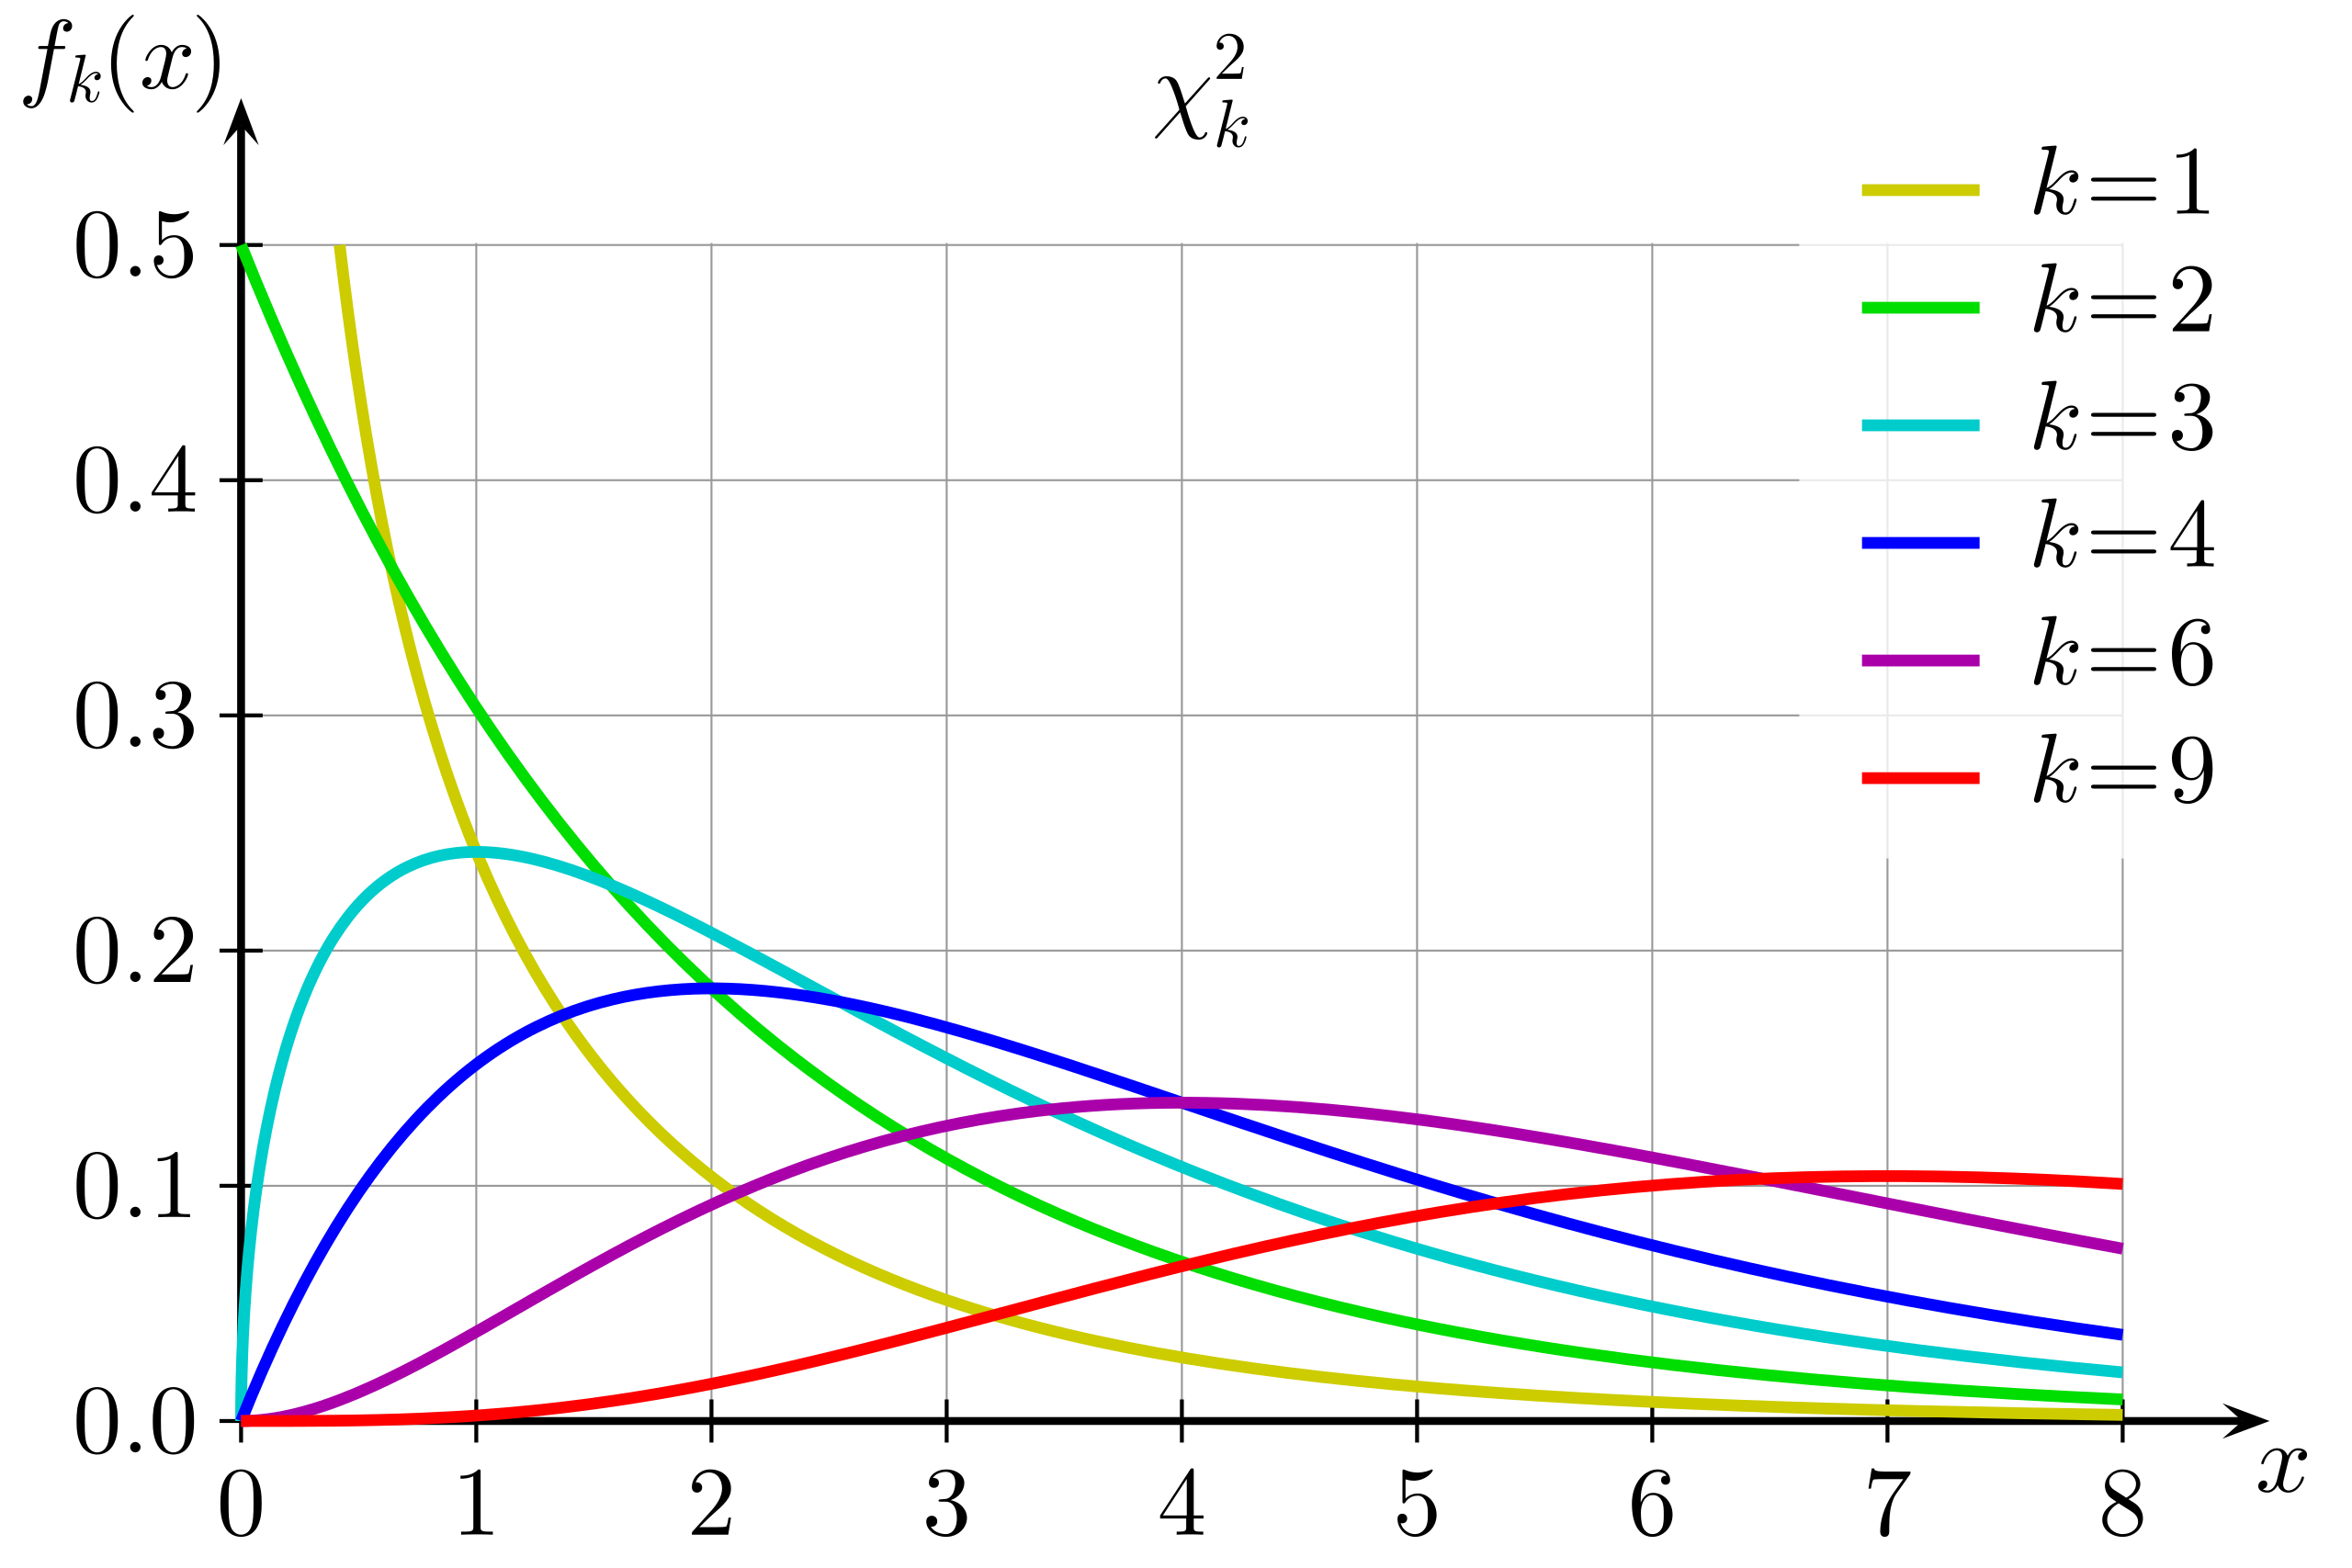
\includegraphics[width=0.5\linewidth]{Chi.png}
    \caption{$k$即为自由度$n$,横轴$x$为随机变量值,纵轴为概率密度}
    \label{fig:Chi}
\end{figure}
可以看到,卡方分布的曲线整体呈左隆起右偏低的态势(随手让你画一个卡方出来,应该都是$k=3$、$k=4$那个样子的),对于卡方的曲线不必有太多记忆,只需要有个初步认识就行(后面要用到分位数的概念),而他有以下几个性质需要牢记,假设卡方分布服从自由度$n$:
\begin{enumerate}
    \item 数学期望为$n$
    \item 方差为$2n$
    \item 可加性,即$\chi^{2}(n)+\chi^{2}(m)=\chi^{2}(n+m)$
    \item (此条感性认识即可)整个曲线位于第一象限,且当$n$趋近于无穷时,卡方分布也就接近正态分布
\end{enumerate}

\subsection{$t$分布}
一句话解释:\textbf{公平较量}。典型式:$\frac{X}{\sqrt{Y/n}}$,记为$t(n)$。其中X表示一个标正态,而Y表示n个标正态的平方和(复习一下,也就是自由度为n的卡方分布)。\par
所以直观上来讲,就是一个分子和分母打架,但是要公平较量的过程。你分母是卡方分布,人多是吧,给我除以n!你平方了是吧,给我开根号!于是这样便得到了t分布。\par
从$t$分布的曲线来看,也是关于$y$轴对称的,长这个亚子:
\begin{figure}[H]
    \centering
    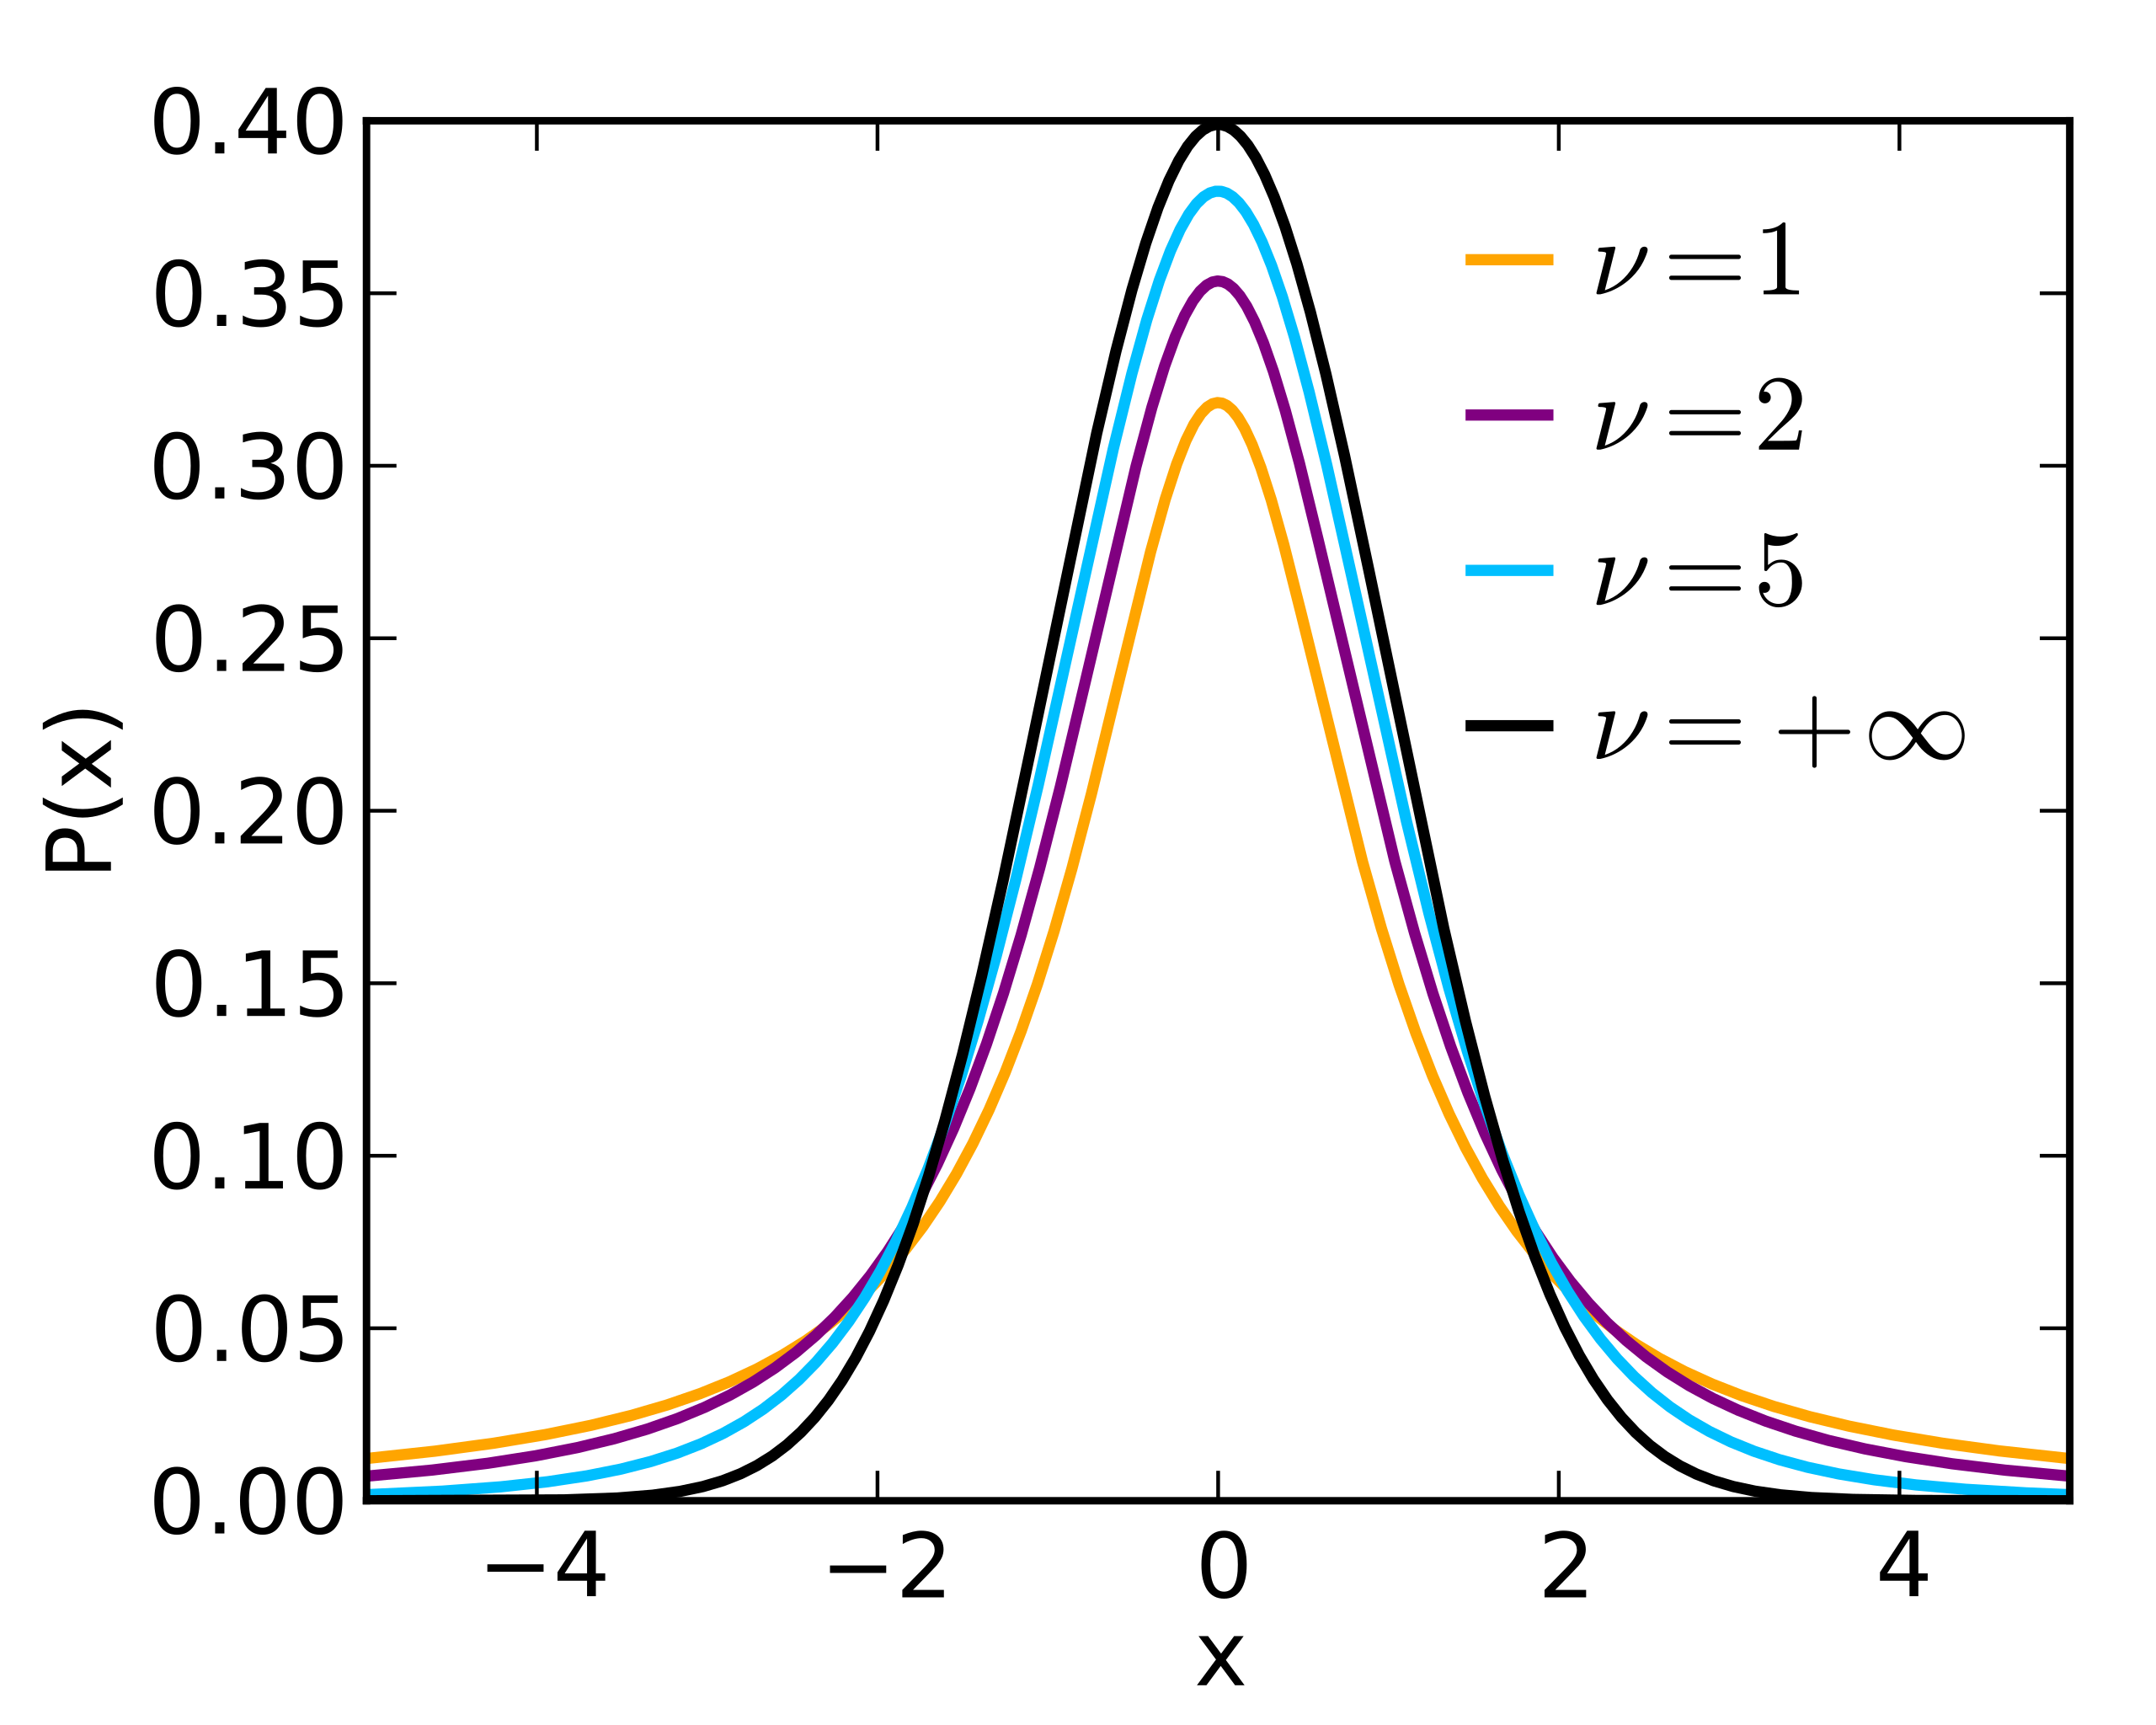
\includegraphics[width=0.5\linewidth]{t.png}
    \caption{$\nu$即为自由度$n$,横轴$x$为随机变量值,纵轴为概率密度}
    \label{fig:t}
\end{figure}
t分布的性质倒不是那么重要,强行列出来几条吧,认识一下就行:
\begin{enumerate}
    \item 关于$y$轴对称
    \item 自由度$n$越大,峰值越高
    \item 当自由度$n$趋近于无穷时,t分布接近于\textbf{标准}正态分布。
\end{enumerate}\par
对称这点比较重要,在之后讨论分位数的概念时会涉及。t分布在历史上是酿啤酒酿出来的(而且就是那个「吉尼斯纪录」的吉尼斯啤酒厂),此后在假设检验中发挥了重要作用,关于其由来感兴趣的同学可以自己查阅。\par
最后冷不丁问个问题,t分布的期望是多少?(笑)

\subsection{$F$分布}
一句话解释:\textbf{打群架}。典型式:$\frac{X/n_1}{Y/n_2}$,记为$F(n_1,n_2)$。其中X表示$n_1$个标正态的平方和(再复习一下,也就是$\chi^{2}(n_1)$),Y表示$n_2$个标正态的平方和(也就是$\chi^{2}(n_2)$)。\par
直观上来讲,这就是t分布的分子来叫了帮手,大家打群架。不过为了防止一方人多,咱们还是来比比平均水平吧。不过这次他们忘了开根号,所以曲线还是像卡方分布一样不太对称(虽然开了根号也不会对称,但大家可以就这么形象记忆)。\par
关于F分布的图像和自身本身的性质都不太重要,重要的是其和另外两个分布的联系。这里还是给出图像给大家一个形象的认识,就类比卡方分布的图像去记忆就可以了:
\begin{figure}[H]
    \centering
    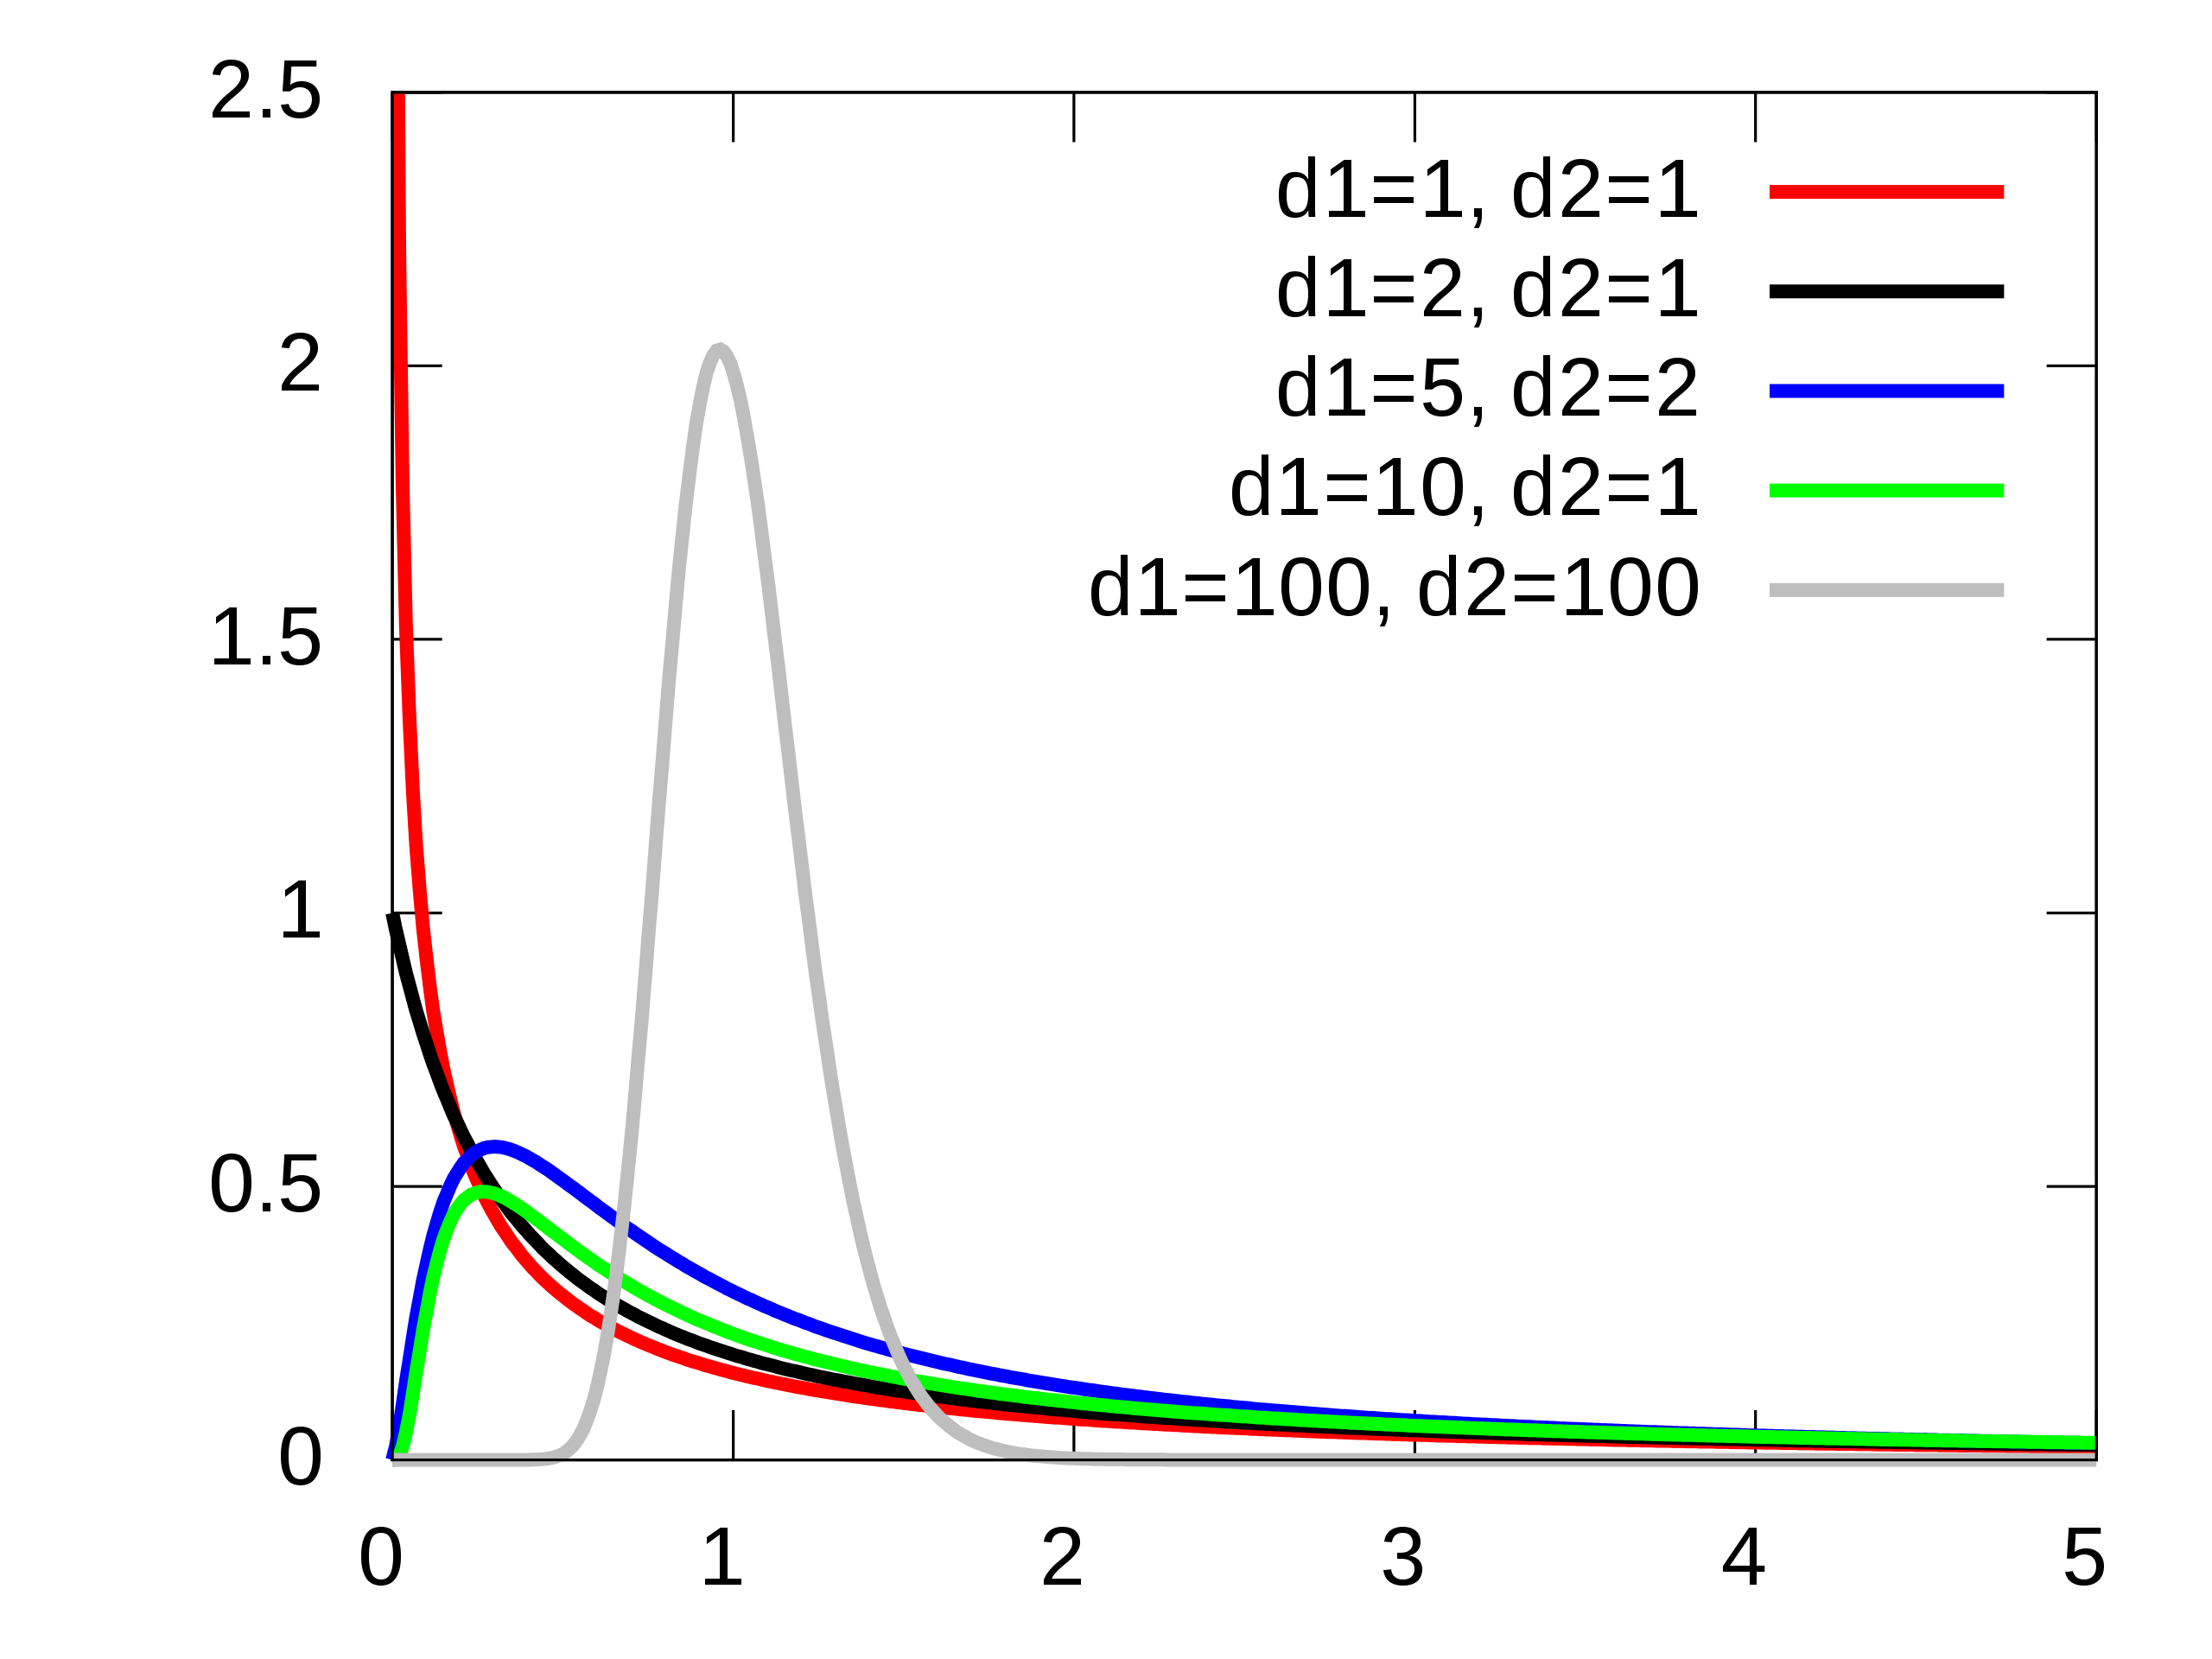
\includegraphics[width=0.5\linewidth]{F.png}
    \caption{$d_1$、$d_2$即为自由度$n_1$、$n_2$,横轴$x$为随机变量值,纵轴为概率密度}
    \label{fig:F}
\end{figure}
比较关键的点在于:
\begin{enumerate}
    \item 若$X\sim F(n_1,n_2)$,则$\frac{1}{X}\sim F(n_2,n_1)$
    \item 若$X\sim t(n)$,则$X^2\sim F(1,n)$
\end{enumerate}\par
关于第二条,就把典型式平方一下就得到了。

\subsection{题目常用结论及注意事项}
\subsubsection{常用结论}
关于此部分内容,如果不会证,就当做一个常用结论记下来(这可是孙老师说的哦),设$\mu$是所服从分布均值、$\sigma^2$是所服从分布方差,那么主要有以下几点是较为常用的:\par
(记住前五条,可以直接用;第六条记不住我们待会儿一起推)
\begin{enumerate}
    \item $\bar{x}$与$S^2$相互独立
    \item $\bar{x}\sim N(\mu, \frac{\sigma^2}{n})$,无论$x$服从什么分布均成立,这是由中心极限定理得到的。
    \item (2.的推论)$\Rightarrow \frac{\bar x - \mu}{\sigma/\sqrt n} \sim N(0, 1)\Rightarrow \frac{(\bar x - \mu)^2}{\sigma^2/ n} \sim \chi^2(1)$
    \item $\frac{1}{\sigma^2}\sum_{i=1}^{n}(X_i - \mu)^2  \sim \chi^2(n)$
    \item $\frac{1}{\sigma^2}\sum_{i=1}^{n}(X_i - \bar x)^2  =\frac{(n-1)S^2}{\sigma^2}\sim \chi^2(n-1)$
    \item $\frac{\bar x - \mu}{S/\sqrt n} \sim t(n-1)$
    \item (6.的推论)$\Rightarrow \frac{(\bar x - \mu)^2}{S^2/n} \sim F(1, n-1)$
    \item (由3.和6.总结的重要推导)$\frac{S}{\sigma}$可做为t分布的分母,自由度为$n-1$
\end{enumerate}
\subsubsection{注意事项}
往往此部分的题目分为两类:
\begin{enumerate}
    \item 证统计量之间的独立性
    \item 会给出一个奇奇怪怪的统计量,然后求证其服从于某个分布(或者给出分布形式,求其系数)
\end{enumerate}\par
对于第一类题目,主要的做法是将其化为$\bar x$、$S^2$等参量,利用已知的相互独立的统计量而推得所求参量独立。如果这条路行不通,可能就要回归原始的求$E(XY)?=EX·EY$(主要用于不等于时证否,等于时只能证不相关)或者求联合概率分布能不能拆开了,一般也不会考到这种程度;\par
对于第二类题目,无论是求解还是求证,总之一定是往这三大分布上凑的。那么具体怎么凑,就要活用\textbf{中心极限定理}了。本次作业的内容解答上很多地方都是直接给结论或者给出一些奇技淫巧的做法,但实际上用中心极限定理去造分布,才应该是解决问题的关键所在,这里我们以上一小节的第六条结论作为例子,尝试证明。\\ \\
\textbf{证:}\par
$易知\bar{x}\sim N(\mu, \frac{\sigma^2}{n})$(结论2,可以直接拿来用)\par
$\Rightarrow \bar{x}-\mu \sim N(0, \frac{\sigma^2}{n})$(接下来我们尝试把分子凑成一个标正态)\par
$\Rightarrow \frac{\bar{x}-\mu}{\sigma / \sqrt n} \sim N(0, 1)$(这里不是中心极限定理,而是方差性质:$D(kx)=k^2D(x)$)\par
$\Rightarrow$ 原式$=\frac{\frac{\bar{x}-\mu}{\sigma / \sqrt n}}{\frac{S/\sqrt n}{\sigma / \sqrt n}}=\frac{\frac{\bar{x}-\mu}{\sigma / \sqrt n}}{\frac{S}{\sigma}}$(下面尝试证分母服从卡方分布开根号)\par
$\qquad \qquad =\frac{\frac{\bar{x}-\mu}{\sigma / \sqrt n}}{\sqrt{\frac{S^2}{\sigma^2}}}=\frac{\frac{\bar{x}-\mu}{\sigma / \sqrt n}}{\sqrt{\frac{(n-1)S^2}{\sigma^2}/(n-1)}}$(往我们熟知的结论上靠)\par
而$\frac{(n-1)S^2}{\sigma^2} \sim \chi^2(n-1)$,故结论得证。\\ \par
总而言之,大家一定要分清楚,什么时候该用中心极限定理(往往是把求和转化为一个分布),什么时候该用方差性质(往往是均值已被化为0,然后把参数作为单独的个体考虑,需要再将方差化为1),结合常用结论凑出目标分布,基本都可以按部就班地解决问题。

\section{分位数与频率替换法}
作业内容参考:1.40、1.41、2.2、2.3\par
本次作业两道是关于分位数的,两道是关于频率替换法的,无论从题目本身还是知识上都比较简单,下面分开介绍。
\subsection{分位数}
所谓分位数的定义就是,随机变量的值小于等于$x_p$的概率等于$p$,我们就把$x_p$这个数(点),称作$p$-分位数(点),我们这里以$\chi^2$分布为例,反映在图像上大致就是这样子的:

\begin{figure}[H]
    \centering
    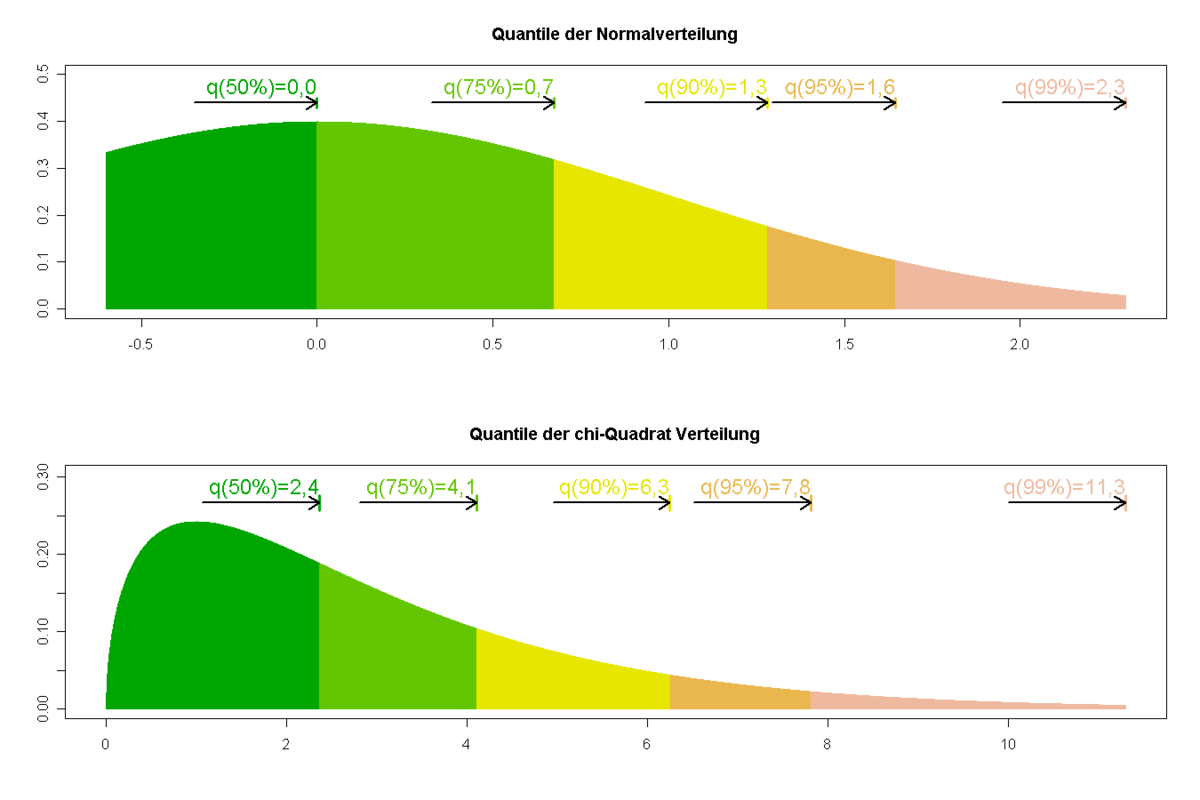
\includegraphics[width=0.8\linewidth]{quantile.png}
    \caption{正态与卡方分布的多个分位点示意图}
    \label{fig:quantile}
\end{figure}
比如最深的绿色那部分区域就已经占到了0.5,深绿与浅绿的分界处就被定义为0.5分位点,依次类推位0.75、0.9、0.95、0.99等分位点。\par
显然,这样的概念是可以落到数学表达式上的。我们前边说到,人类对三大分布加上正态分布的了解已经非常充分了,是的,这种充分程度也包括对这些分布的分位数。也就是说,比如我想求$\chi^2(n)$分布的0.86分位点(我随便说的一个数),就可以通过查表来获得,因为这些分布都是确定的,他们的分位点自然也就确定了。也因此,统计学家们可以\textbf{将未知分布转化为这四大分布}的分位数,以迅速得到他们想要的统计信息,而这其实也正是我们做题的核心思路。\par
下面给出四个(也就是四大分布)我们认为是已知的分位数表示:
\subsubsection*{标准正态分布}

\begin{center}
    $P\left(x \leq {\textcolor{magenta}{z_p}} \right)=p$   
\end{center}\par
且有$-z_p = z_{1-p}$.

\subsubsection*{$\chi^2$分布}

\begin{center}
    $P\left(\chi^2 \leq {\textcolor{magenta}{\chi^2_p (n)}} \right)=p$   
\end{center}\par

\subsubsection*{$t$分布}

\begin{center}
    $P\left(T \leq {\textcolor{magenta}{t_p (n)}} \right)=p$   
\end{center}\par
$t$分布关于$y$轴对称,故有$- t_p (n) = t_{1-p} (n)$.

\subsubsection*{$F$分布}

\begin{center}
    $P\left(F\leq {\textcolor{magenta}{F_p (n_1, n_2)}} \right)=p$   
\end{center}\par
且有$F_p (n_1, n_2) = \frac{1}{F_{1-p} (n_2, n_1)}$.\\\par

以上四个标粉色的量都被认为是“已知的”,所以如果题目要你求一个什么统计量的分位数,就尽量利用1)概率内部的不等式变形或2)以上三个小等式进行转化,然后最后用这四个已知量去表示即可。\par
最后需要注意的一点是,我们这里以$\chi^2$分布为例,假设其服从自由度$n$。如果我们得到一个等式:
\begin{center}
    $P\left(\chi^2 \leq k x_p \right)=p$   
\end{center}\par
其中$x_p$是我们要求的原统计量的分位数,现在我们通过不等式变形得到了这个结果,这个时候我们根据$\chi^2$分布的已知量应该得到的等式是$\chi^2_p (n) = k x_p$,终而得到$x_p = \frac{1}{k} \chi^2_p (n)$为所求。你可千万不要搞出个什么$\chi^2_{k x_p} (n)$这样令人啼笑皆非的东西哈,切记分位数是针对于比例(或者我们之后要学习的置信度)而言的。

\subsection{频率替换}
频率替换这个东西就很简单了,其理论基础就是大数定律,思想核心就是\textbf{通过频率来替换概率}。比如我们抛10000次硬币,其正面朝上的频率,应该能很好地反映出我抛1次硬币正面朝上的概率,这就是频率替换法,也是前面提到的「频率派」的主要武器。\par
对于此类问题,题目都会很显式地给出类似于“在这$n$个样本观察值中有$m$个取值小于2(发生某个事件)”这样的话,那么这就很清楚了:$\frac{m}{n}$对应的就是频率,所要替换的就是它所观察对象(发生某个事件)的概率,在这句话中就是“取值小于2”这个事件。\par
也即是说,我们应该假设控制分布的参数$\theta$已知,然后计算出“取值小于2”的、用$\theta$表达的数学期望。如果说这个事件发生的概率是$p$,那么$p$应该等于这个数学期望,我们反解出用$p$表示的$\theta$,再用频率$\frac{m}{n}$替换掉概率$p$,我们就可以美其名曰,只要做个实验,我们就可以通过实验得到的频率,来很好地估计未知参数了。\\\par

\textbf{一个简单的栗子.}我们假设一个运动员打靶服从于两点分布$B(1,\theta)$,即击中概率为$\theta$,不击中概率为$1-\theta$。现在我们让运动员进行100次训练,每次训练打靶10次,在这100次训练中观察到有50次训练都全部中靶,试求$\theta$的频率替换估计?\par
显然,这里的频率就是$\frac{50}{100}=\frac{1}{2}$,而对应的事件应该是“全部中靶”,这个事件的数学期望应该是$\theta^{10}$。假如说全部中靶的概率为$p$,那么应该有$p=\theta^{10}$;反解得到$\theta = p^{\frac{1}{10}}$,然后用频率$\frac{1}{2}$去替换概率$p$,即可得到$\theta$的频率替换估计为$2^{-\frac{1}{10}}$。(顺手用计算器算了一下这个概率约等于0.933,好像还挺合理的)\\\par

最后,我们以这个朴素的方法来为本章拉开一个序幕。所谓参数估计,它的核心思想就是通过抽样后得到的统计量,来推断分布中的参数。在频率替换法中,是利用频率来替换概率并推断参数;在后面的矩估计中,则是通过矩来替换;再之后的最大似然估计,则是通过最大化似然函数,他们都难逃「频率派」的核心假设,即参数本身是确定的,我只要做实验,就可以去逼近、推断参数。\par
但相对而言这又是一个比较“蠢”的方法。「贝叶斯派」会反唇相讥:你怎么知道这个试验是服从这个分布的?又是怎么知道未知参数的个数的?这在具体问题中,对于那些未知数据是很难做出判断的。不过,从古典的眼光审视,我们也并不能否认其在应用上的广泛性,对于大部分实际问题,我们都能很好地用一些已知分布去刻画,这背后或许是中心极限定理的功劳,但也不妨视此为一种大自然的馈赠吧。

\section{矩估计和极大似然估计}
作业内容参考:2.5、2.8、2.10、2.11、2.12、2.15\par
首先做一个声明,在数理统计中我们不一般不对“最大”和“极大”做区分。续接上一节,我们可以把矩估计看作为一种更高端的替换方式,而把极大似然估计(Maximum Likelihood Estimation, MLE)看作是一种更高端的求参方式(不用反解,改求导了)。两种方法的思想也都很朴素,做法也都很循规蹈矩,但是在实际使用中其实有很多要注意的细节,请读者务必重视。
\subsection{矩估计}
受辛钦大数定律(不知道也没关系)的启发,我们可以通过\textbf{矩}来估计参数。而矩又分为原点矩和中心矩,每一种矩又区分为样本~矩或总体~矩。首先给出矩的相关定义(如果只从会做题的角度出发,以下概念都不用记住):

\subsubsection*{$k$阶原点矩}
\begin{center}
样本:$A_k=\frac{1}{n}\sum_{i=1}^{n}x^k_i$ \\
总体:$E(X^k)$
\end{center}
\subsubsection*{$k$阶中心矩}
\begin{center}
样本:$B_k=\frac{1}{n}\sum_{i=1}^{n}(x_i - \bar x)^k$ \\
总体:$E[(X - E(X)]^k$
\end{center}\par
显然,特殊情况时一阶\textbf{原点矩}对应样本均值,二阶\textbf{中心矩}对应样本方差。总结来说,原点矩是$x_i$关于原点(0)的差值,中心矩是$x_i$关于$\bar x$的差值,k阶即对应k次方。无论是使用原点矩还是中心矩做参数替换都是可以的,一般来讲都使用总体原点矩,因为好求。\par
更具体地,我们求出的某阶总体矩(比如一阶总体原点矩,也就$\mu$或者说$\bar x$),它一般是一个带有未知参数$\theta$的表达式;而这之后就和频率替换的方式完全一致,即通过反解得到$\theta$关于矩或者统计量的表达式,这就是对参数的矩估计。\par
于是,就有一个很关键的原则了:\textbf{有几个未知参数就要求几阶矩}。所以矩估计也是一个很套路的事情,总结如下:
\begin{enumerate}
    \item 检查有几个未知参数(题目一般会问,求某个或某几个参数的矩估计)
    \item 计算对应的几阶矩。一般都是一阶原点矩也就是$E(X)$,如果两阶就是$E(X)和E(X^2)$或者$E(X)和D(X)$(二阶中心矩),看求哪个方便。三阶情况除非是做梦才会考,但原理也是相通的。
    \item 一阶情况,反解,使用E(X)表示参数;二阶情况,列方程组解出参数
    \item 使用对应的统计量替换期望或者方差,比如$\bar x$或$\sigma^2$;如果没有对应的统计量,直接用$A_k$或者$B_k$表示$k$阶原点/中心矩也是可以的
\end{enumerate}
\par
最后补充一点,孙老师说有一年就特意考了一个一阶矩估计不出来参数的情况,学生们就傻了。如果遇到这种情况,就继续求二阶矩,总之求到可以表示出参数为止。
\subsection{极大似然估计}
对于考研学生来讲,极大似然估计应该是基本功了,毕竟是十分大题,基本就是送。但我估计很多人也是知其然不知其所以然,所以我们这里着重讲一下MLE(指代极大似然估计,下同)的理解和与研究生考试相区别的地方。\par
首先,什么是似然(Likelihood)?\par
通俗地讲,似然就是通过样本的数据,反过来估计真实模型\textbf{最可能的情况}。\par
比如抛一枚硬币,十次全是正面朝上,那么likelihood is这个硬币有问题。\par
再比如,一个盒子里有黑球和白球,我们需要考察黑球和白球的比例,这时我们对盒中的球进行100次有放回的抽取,有70次抽到黑球,30次抽到白球,那么likelihood is黑球和白球的比例是7:3(不信你们可以用MLE求一下)。\par
于是,MLE的核心要素在于:令抽样事件发生的概率最大,此时的参数即为MLE。定义似然函数:
\begin{center}
    $L(\theta;x_1,x_2,...,x_n)=\prod _{i=1}^n p(x_i,\theta)$
\end{center} \par
那么使抽样事件发生的概率最大,就以为似然函数最大,也就是我们只需要对似然函数关于参数求导即可。而往往连乘操作易造成下溢,所以通常取对数似然(log-likelihood),两者具有相同的极值点:\par
\begin{center}
    $\ln L(\theta;x_1,x_2,...,x_n)=\sum _{i=1}^n \ln p(x_i,\theta)$
\end{center} \par
这样的形式往往更易于求导。另导数为零,此式接触的参数值即为MLE。所以MLE也是一个很套路的事情,我们在这里总结一下:\par
\begin{enumerate}
    \item 求出似然函数,也就是概率密度函数的连乘
    \item 如果指数函数比较多,就继续写出对数似然函数
    \item 对似然函数求导,化简
    \item 另导数为零,解出参数值即为所求
\end{enumerate} \par
这里有两个需要注意的点:\par
\begin{enumerate}
    \item 如果未知参数多于两个,就分别对两个参数求导,这样会得到方程组从而求解。这样的原理大致可以理解为(以两个未知参数为例),参数A的极值是关于参数B的函数,参数B的极值又是关于参数A,讲道理此时应该继续求二阶导,但往往这样的问题会有一个参数先确定下来从而另一个也就确定了,如果没有的话不妨求二阶导讨论一下,这里存疑,因为我看作业题并没有求二阶导。
    \item 第二个关键的问题就在于,\textbf{驻点不一定在参数取值范围内!}因为这个事儿孙老师还特意拿出了某年考研题出来鞭尸,说判了五天卷子最后一天发现极值点不在参数范围里……
\end{enumerate} \par
这是研究生学习和本科学习中区别较大的一点。在解出参数值之后一定要讨论驻点是否在参数范围内,往往要分在与不在讨论。这里以2.12作为栗子进行讨论。\\\par

\textbf{一个不太简单的栗子.}从一个正态总体$N(\mu, \sigma^2)$中取样得到$x_1,x_2,...,x_n$,$\mu$和 $\sigma^2$都是未知参数,且$\mu \leq \mu_0$(注意这里,这就是研究生和本科的区别。。),其中$\mu_0$是已知常数,试求$\mu$和$\sigma^2$的MLE?\\\par
前边那些基操在这里就都略过了,因为闭着眼都知道,其实无论是什么分布,你均值的最大似然一般都是均值啊($\mu$的最大似然是$\bar x$),方差的最大似然都是方差啊($\sigma^2$的最大似然是$\frac{1}{n} \sum_{i=1}^n (x_i-\bar{x})^2$)这一点想想就很合理哈哈哈。\par
那假装我们求出了MLE是以上表达式,这是区别的地方就是,我们需要讨论这个$\bar x$是否在范围当中。在这里就是它特意给了个$\mu \leq \mu_0$。那么如果:
\begin{enumerate}
    \item $\bar{x}$确实小于$\mu_0$,显然驻点为所求,作答。
    \item 如果$\bar{x}$大于$\mu_0$,这时我们就要回到似然函数的导数去,看看似然函数关于参数的增减情况了。在讨论的时候,我们需要固定一方而讨论另一方,比如这里就是,在给定$\sigma^2$的情况下,$\mu$的变化对于似然函数的变化是什么?反之在给定$\mu$的情况下,$\sigma$的变化对于似然函数的变化又是什么?
\end{enumerate} \par
当然了,这里有一个\textbf{很投机取巧的方法}:选择两者其中那个带有约束的参数(在例子中就是$\mu$),先讨论下来这个参数的MLE(比如这里答案就是先讨论了$\mu$,确定了在情况2下,$\mu$的MLE就是$\mu_0$),那么此时就可以回到另一个参数在驻点中的表达式,直接确定另一个参数(因为没有约束嘛,可以理解为只与有约束的那个参数相关)。\par
总而言之,大家在走完套路之后,一定要记住检查驻点的范围,考到就是赚到,哈哈哈。\par

\section{无偏估计}
作业内容参考:2.20、2.22、2.25\par
本节内容都是关于无偏估计的。这一节内容相对来讲比较简单,因为主要是给后面的UMVUE等内容做铺垫。所以恭喜你,这一节的内容很快就可以学完,但这只是暴风雨前的宁静啊……\par
\subsection{无偏性}
简言之,如果~某个统计量的数学期望~等于~关于未知参数的某个函数~,那么这个统计量就是这个函数的\textbf{无偏估计}。形式化地表达就是:
\begin{center}
    $E_\theta (T(X))=q(\theta)$
\end{center} 
\par
\textbf{一个炒鸡简单的例子.}考虑一个两点分布$B(1,p)$,进行抽样,请问样本均值$\bar x$是否为参数$p$的一个无偏估计?\\\par
答:想要论证这一点,只需要求$E(\bar x)=1·p+0·(1-p)=p$,发现确实等于$p$,所以是一个无偏估计。所以考无偏估计,无外乎三种考法:
\begin{enumerate}
    \item 论证是否存在无偏估计
    \item 判断某统计量是否是无偏估计
    \item 找出一个无偏估计
\end{enumerate}\par
1.和3.相对于2.而言肯定更难一些,不过大体思路也是一致的。\par
对于第一点,无偏估计一般是存在的,甚至一般来讲是不唯一的,所以要想论证存在,实际上等价于3.,如果要论证不存在,往往是些极端情况,使用反证法破之即可。\par
对于第二点,求个期望就出来了,不再赘述。所以我们还是主要来关注一下3.。To the best of my knowledge,找出一个无偏估计,一般要向k阶矩去靠。比如求$p$的无偏估计,我们就试试一阶矩,求$p^2$的我们就试试二阶矩,$p^3$、$p^4$等依此类推。有的时候会出现那种一阶矩就出来二次方的情况,但反正往矩,也就是均值、方差等上靠总是没问题的,这样求出来一般是待求参数(函数)的某个带有常系数的兄弟,所以我们也对应地在统计量中添加常系数修正就好了(比如修正样本方差就是这么来的)。\par
此外,如果某些时候k阶矩求出来是个“混合体”,比如是个什么$c_1 p+c_2 p^2$的东西,我们又想求$p^2$的无偏估计,我们这个时候就可以发挥转化思想,将问题转化为求$p$的无偏估计(一般来讲,在更低阶的矩里你已经求出来了),求出后我们再用k阶矩去减就可以了,乘除什么的也可以以此类推(虽然一般可以平方开根号之类的),这样就解决了问题。总之,求无偏估计是一个在套路之外稍微考察一些代数式恒等变形能力的问题,从这一点来看,他可比矩估计高到不知道哪里去了。
\subsection{更好的无偏估计}
前文说过,无偏估计一般存在,且一般不唯一。所以这个时候就有一个很自然的问题:哪个更好?\par
所以其实也有一个很自然的想法就是:虽然你期望估计是相同的,但是方差估计呢?于是考虑更好的无偏估计的做法,就是将这两个\textbf{无偏估计量}(之所以加粗,是因为他们首先必须是无偏估计,才能判断谁更好,这是个大前提)的方差求一求,比比谁的方差更小,谁就是更好的无偏估计。对于方差的求解一般是利用$D(X)=E(X^2)-[E(X)]^2$这个公式,想必大家也不陌生了,在此就不赘述了。
\end{document}